\documentclass[main.tex]{subfiles}
\begin{document}
\begin{titlepage}

\newcommand\BackgroundPic{\put(0,0){\parbox[b][\paperheight]{\paperwidth}{\vfill \raggedright 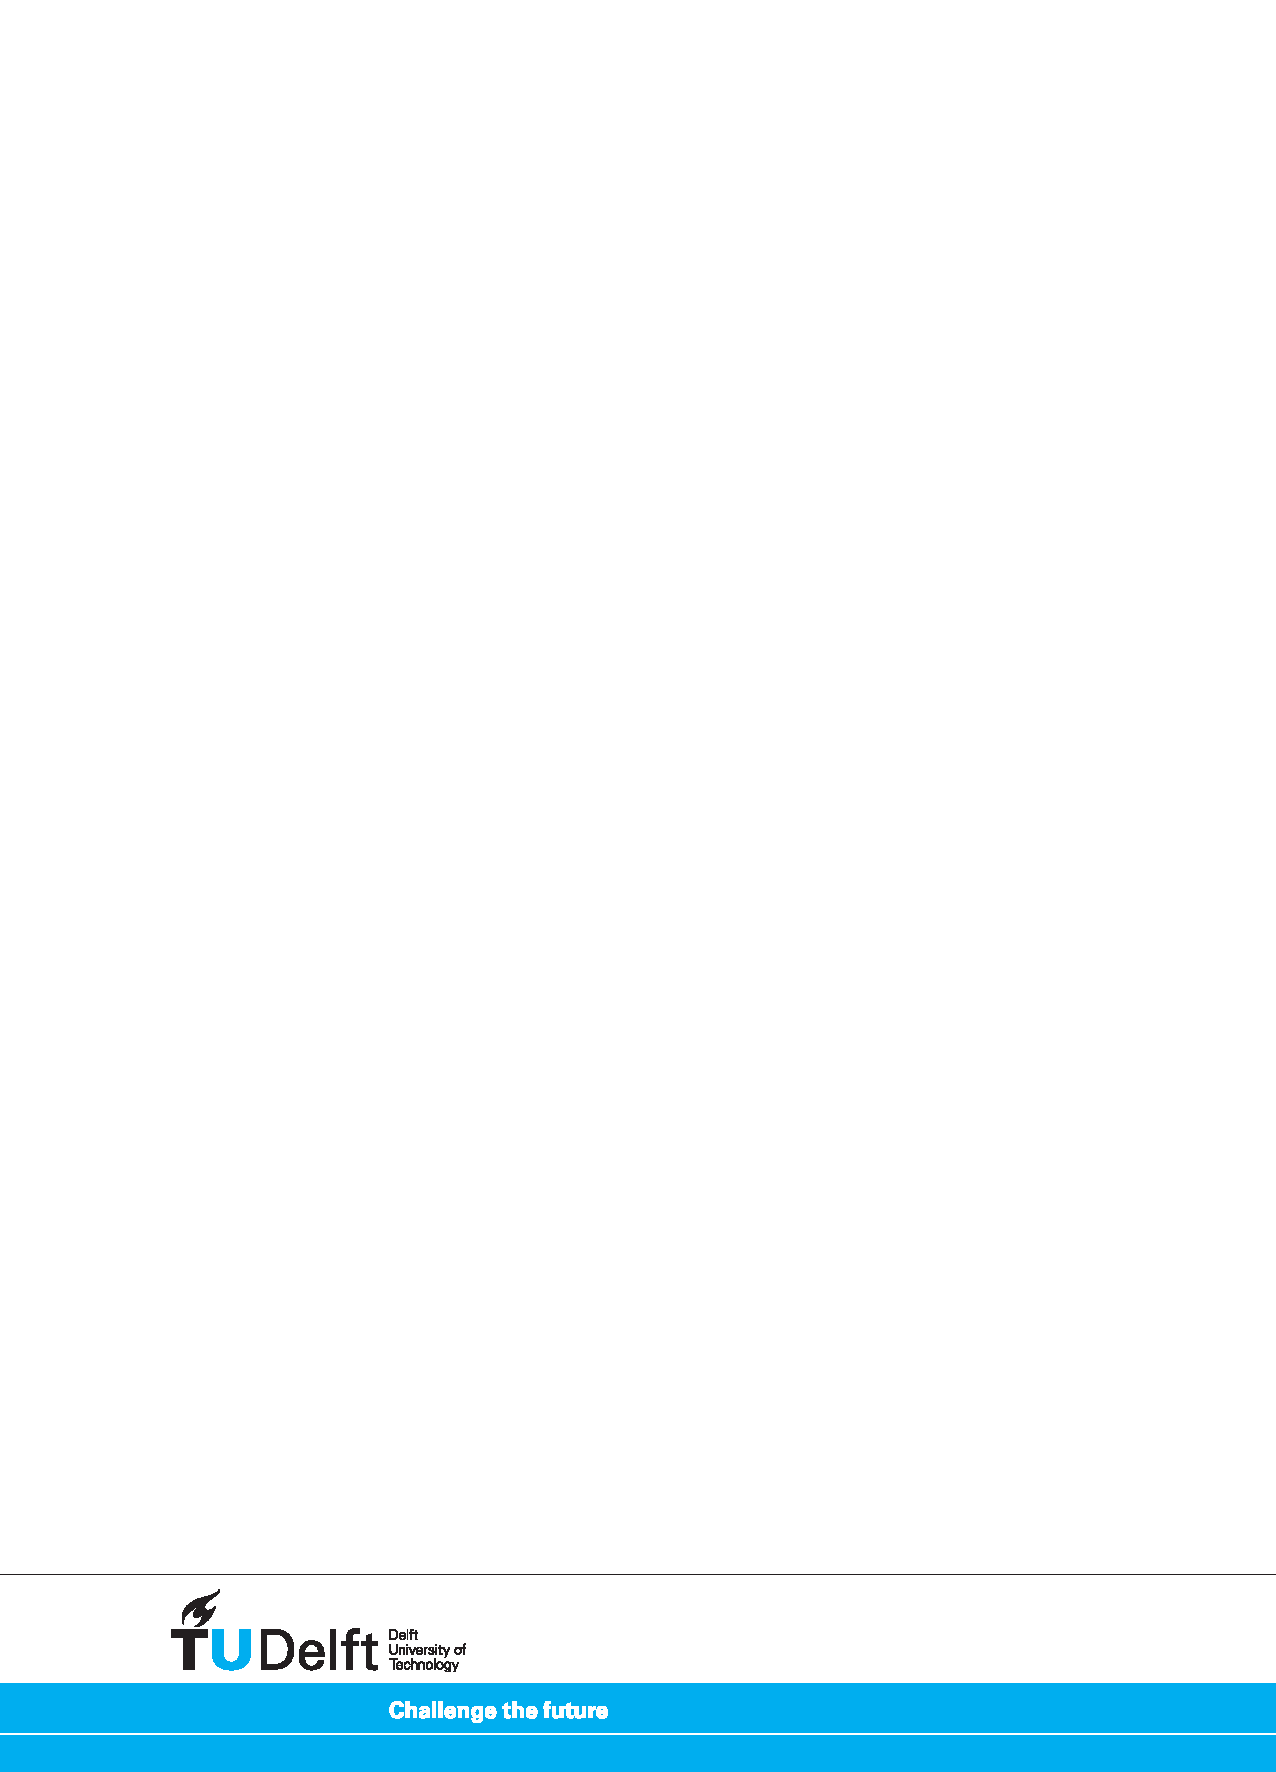
\includegraphics[width=\paperwidth,height=1.05\paperheight]{./Images/TUDelft_border.pdf}}}}
\AddToShipoutPicture*{\BackgroundPic}

\begin{center}
    \noindent\makebox[\linewidth]{\rule{\textwidth}{1pt}}
    \smallskip
    \begin{Large}
    \textbf{Assignment - 3\\Re-Design of an Airfoil}
    \end{Large}
    \textit{\\\vspace*{0.3em}AE4130 - Aircraft Aerodynamics\\}
    \today \\
    \noindent\makebox[\linewidth]{\rule{\textwidth}{0.1pt}}
\end{center}
\vspace{2cm}

\begin{figure}[h!]
\centering
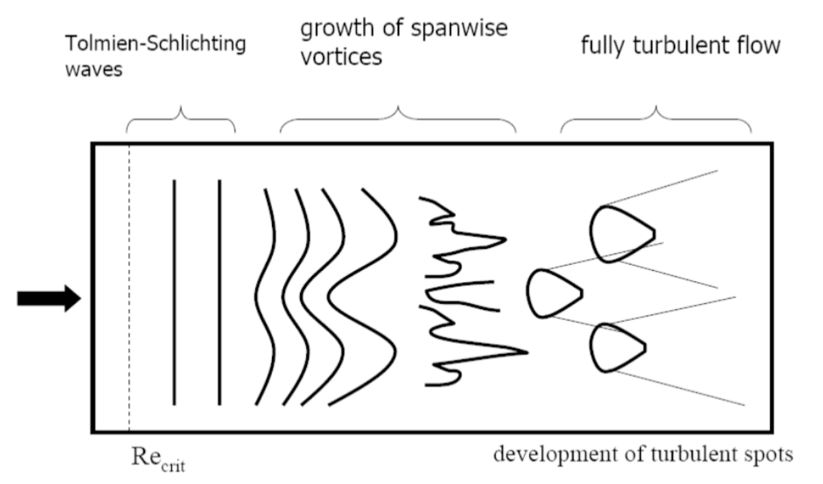
\includegraphics[scale=0.6]{./Images/Ass3/FrontPage}
\end{figure}
\centering
Boundary Layer Tansition Process taken from \textit{[AAP-Handout \#1, L.L.Veldhuis, 2014]}
\vfill
\begin{flushleft}
    \smallskip
\vspace*{2\bigskipamount}
    \textbf{Supervisor:\\}
    Prof.dr.ir. L.L.M. Veldhuis \\\vspace*{0.8em}
    \textbf{Particiants:\\}
    A.G. Monikantan $|$ 4738942\\
   
% \noindent\makebox[\linewidth]{\rule{\textwidth}{1pt}}
    \vspace{1cm}
\end{flushleft}
\end{titlepage}
\end{document}
